\documentclass{article}
\usepackage{graphicx} % Required for inserting images
\usepackage[ngerman]{babel}
\usepackage{enumitem}

\title{Pflichtenheft \\ \large Einflussfaktoren auf die Verkehrsmittelwahl\\ -- Baukasten für Discrete Choice Modelle}
\author{Kevin Boehnke \\ \texttt{uxpkw@student.kit.edu}
\and Floriane Bresser \\ \texttt{uspvq@student.kit.edu}
\and Damian Reich \\ \texttt{uqppn@student.kit.edu}
\and Alissa Saleh \\ \texttt{unmbc@student.kit.edu}
\and Michael Schur \\ \texttt{ufkmz@student.kit.edu}}
\date{24. Mai 2023}

\begin{document}
\clearpage\maketitle\thispagestyle{empty}
\newpage
\clearpage\tableofcontents\thispagestyle{empty}
\newpage
\pagenumbering{arabic}

\section{Einleitung}

\section{Zielbestimmung}
Das Produkt soll die Verkehrsingeniure dabei unterstützen, Verkehrsmodelle zu erstellen, modifizieren und visualisieren.
\subsection{Musskriterien}
\begin{itemize}
    \item[\textbf{/MK1/}] Der Nutzer kann Erhebungsdaten im CSV-Format importieren.
    \begin{itemize}
        \item Die Spaltennamen können sich zwischen Tabellen unterscheiden.(?)
    \end{itemize}
    \item[\textbf{/MK2/}] Der Nutzer kann Tabellen durch Attributsableitungen erweitern.
    \subitem Folgende Möglichkeiten stehen dem Nutzer zur Verfügung:
    \begin{itemize}[leftmargin=.7in]
        \item[\textbf{/MK2.1/}] Intervalle
        \item[\textbf{/MK2.2/}] Gruppen
        \item[\textbf{/MK2.3/}] Logische Ausdrücke
        \item[\textbf{/MK2.4/}] Vergleiche
    \end{itemize}
    \item[\textbf{/MK3/}] Der Nutzer kann Nutzenfunktionen für alternative Verkehrsmittel definieren.
    \begin{itemize}[leftmargin=.7in]
        \item[\textbf{/MK3.1/}] Der Nutzer kann Linearkombinationen für die Nutzenfunktion verwenden.
    \end{itemize}
    \item[\textbf{/MK4/}] Der Nutzer kann die Parameter und Signifikanz aus gegebener Eingabe und Modellstruktur berechnen lassen.
    \item[\textbf{/MK5/}] Das Programm bietet eine Schnittstelle für andere Bibliotheken zur Parameterschätzung und Signifikanzgewinnung. 
    \begin{itemize}
        \item Es wird standardmäßig das Python Paket \textit{Biogeme} verwendet.
    \end{itemize}
    \item[\textbf{/MK6/}] Das Programm visualisiert die gewonnenen Parameter und Signifikanzniveaus.
    \item[\textbf{/MK7/}] Das Programm bietet eine Schnittstelle(?) um die Parameteraufteilung zu erweitern oder einzuteilen anhand der Signifikanzniveaus.
    \item[\textbf{/MK8/}] Nutzereingaben(?) können gespeichert und geladen werden.
\end{itemize}

\subsection{Wunschkriterien}
\begin{itemize}
    \item[\textbf{/WK1/}] Das Programm unterstützt arbiträre Funktionen in der Attributaufbereitung.
    \item[\textbf{/WK2/}] Die vom Nutzer definierten Funktionen können gespeichert werden.
    \item[\textbf{/WK3/}] Der Nutzer wird bei der Programmführung durch folgende Funktionen von der Software unterstützt:
    \begin{itemize}[leftmargin=.7in]
        \item[\textbf{/WK3.1/}] Autovervollständigung
        \item[\textbf{/WK3.2/}] Typhinweise
        \item[\textbf{/WK3.3/}] Fehlerunterbindung
    \end{itemize}
    \item[\textbf{/WK4/}] Die Nutzenfunktionen im Modell-Aufbau können wie folgt verschachtelt werden:
    \begin{itemize}[leftmargin=.7in]
        \item[\textbf{/WK4.1/}] Arithmetik: $\beta \cdot (T + (\beta_2 \cdot X_2 \cdots))$
        \item[\textbf{/WK4.2/}] Exponentialfunktionen: $\log(T)$, ${\rm e}^T$
        \item[\textbf{/WK4.3/}] Potenzen: $\beta \cdot X^3$
    \end{itemize}
    \item[\textbf{/WK5/}] Das Programm kann um andere Modell-Strukturen, wie beispielsweise Nested Logit, erweitert werden.
    \item[\textbf{/WK6/}] Der Nutzer kann die Schwellwerte für die Signifikanz selber konfigurieren.
    \begin{itemize}
        \item Beispiel bei Apollo: $|T-Ratio | > 1.95$, $|Robust T-Ratio | > 1.95$
    \end{itemize}    
    \item[\textbf{/WK7/}] Es existiert ein vollwertiger Algorithmus zur Bestimmung von Signifikanzgruppen und Aufteilungen
    \item[\textbf{/WK8/}] (Intuitive UI)
    
\end{itemize}
\subsection{Abgrenzungskriterien}
    
\section{Produkteinsatz}
\subsection{Anwendungsbereiche}
\begin{itemize}
    \item In der Verkehrsbereich und in der Recherche
\end{itemize}
\begin{itemize}
    \item Prognose und quantitative Basis für verkehrsplanerische, (betriebswirtschaftliche) und politische Entscheidungen?
\end{itemize}
\subsection{Zielgruppen}

\begin{itemize}
    \item Verkehrsingenieure und Verkehrswissenschaftler
    \item Keine Informatiker (außer um Code zu erweitern)
\end{itemize}
  
\subsection{Betriebsbedingungen}

\section{Produktumgebung}
\subsection{Software}
\begin{itemize}
    \item Die Software wird in Python geschrieben.
    \item Betriebssystem: Windows 10 oder Windows 11
    \item Die Software wird als Open Source veröffentlicht und erweiterbar sein.
\end{itemize}
\subsection{Hardware}
\begin{itemize}
    \item Das Produkt ist eine Desktopanwendung.
    \begin{itemize}
        \item Mindestanforderung: Laptop, 8GB RAM, Intel Core i5 (4 Kerne, 8 logische Kerne)
        \item \textit{WK}: Workstation, Windows Server, 8 Kerne (16 logische Kerne)
    \end{itemize}
\end{itemize}
\subsection{Schnittstelle}
\begin{itemize}
    \item Die Software nimmt Dateien im CSV-Format entgegen.
    \item \textit{WK}: Die Anwendung soll über eine Schnittstelle andere Bibliotheken zur Parameterschätzung einbinden können.
    \begin{itemize}
        \item beispielsweise das \textit{Apollo Package}
    \end{itemize}
\end{itemize}
\newpage

\section{Produktfunktionen}
\subsection{Funktionsübersicht}
Im folgenden ist eine Übersicht der Produktfunktionen
\begin{center}
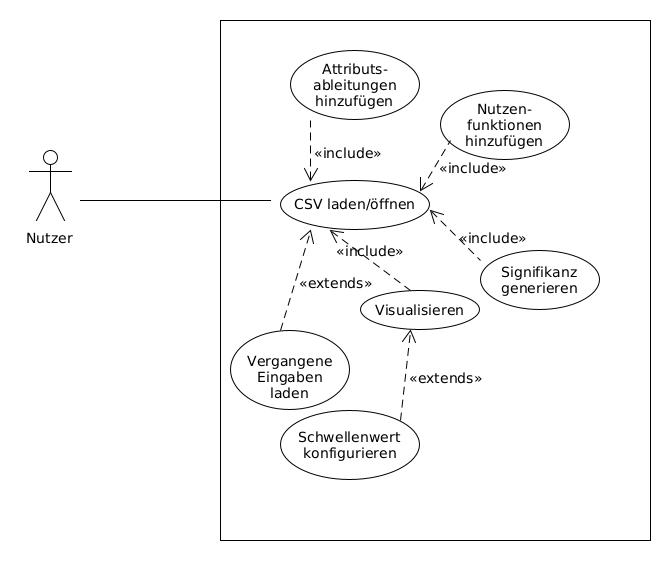
\includegraphics[width=10cm]{use case2.jpg}\\ 
\caption{Abb. 1.0: Use Case Diagramm} 
\end{center} 
\textbf{F10} Erhebungsdaten lesen \\
\textbf{F15} Attributsableitungen hinzufügen \\
\textbf{F20} Nutzenfunktionen eingeben \\
\textbf{F25} Signifikanzgenerierung \\
\textbf{F30} Visualisieren \\
\textbf{F35} Schwellwerte konfigurieren
\subsubsection*{F10 Erhebungsdaten lesen}
\underline {Ziel}   Bereits existiernde CSV Datei öffnen, welche die nötigen Erhebungsdaten beinhaltet

\section{Produktdaten}

\section{Produktleistungen}

\section{Benutzungsschnittstelle}

\section{Globale Testfälle}

\section{Qualitätsbestimmung}

\end{document}
